\chapter{\attekintes}

Egy adatbázisnak sok része tesztelhető, ezek közül az alábbi három az ami a kutatásom témájába vág:
\begin{itemize}
	\item  \textbf{A lekérdezéseket beolvasó editor tesztelése}: Az editor sok szempontból lehet hibás. Funkcionális szempontból az editor által elfogadott lekérdezések halmaza eltérhetnek a specifikációban leírtaktól például egyes a specifikáció alapján felírt nyelvi konstrukciókat az editor nem fogad el. A dologozatban bemutatott módszerrel például felfedeztem, hogy a Neo4j  editora csak olyan lekérdezéseket hajlandó beparszolni, amelyekbe, egy referencia csak egyszer szerepel a visszatérési értékben. (\cypherStyle{RETURN V1, V1} nem fordul). Ezen kívül az editorok nagy és bonyolult programok, ezért egy-egy fejlesztési lépés után drasztikusan lelassulhatnak.\footnote{Editor terribly slow - \url{https://www.eclipse.org/lists/viatra-dev/msg00501.html}}\footnote{Type inferrer is slow because of repeated calculations of single compatible parent type - \url{https://bugs.eclipse.org/bugs/show_bug.cgi?id=534807}}
	\item \textbf{A lekérdezések feldolgozása}: Lekérdezés optimalizáló, lekérdezési terv készítő vagy típuskövetkeztető tesztelése. Ilyenkor egy lekérdezés esetén azt vizsgáljuk, hogy a lekérdezésnek megfelelő/optimális/köztes struktúra jön-e létre.
	\item \textbf{Lekérdező motor tesztelése}:  Célja az, hogy meghatározzunk a lekérdező motor helyes eredményt ad-e vissza, egy lekérdezésre. Többféle megközelítésben lehet összehasonlítani a helyességet : (1) Más adatbázis implementációkkal (2) A lekérdező rendszer korábbi verziójával (Regressziós tesztelés) \cite{yan2018snowtrail} (3)Egy összetettebb tesztorákulummal \cite{DBLP}. Munkám elsődleges célja ez.
\end{itemize}



\section{Funkcionális áttekintés}

Munkám célja hogy elkészítsek egy olyan megközelítést, amely képes gráflekérdezések automatikus generálására, gráfmintaillesztő rendszerek tesztelése. Az elképzelt  keretrendszer koncepcionális elrendezését  \aref{fig:funkcionalisAttekintes} ábrán mutatom be. Az ötlet lényege az, hogy a tesztelni kívánt rendszer \textbf{nyelvi specifikációjának} és egy \textbf{esettanulmány szignatúrájának} (ezalatt egy olyan tulajdonsággráf adatmodell alapú adatbázis szignatúrájára gondolok amely az adott lekérdező rendszert használja) bemenetként való felhasználásával, a kimeneten szöveges és a gráfmintaillesztő rendszer nyelvén íródott lekérdezéseket kapjak. 

Amint rendelkeznék egy tesztkészletnyi ilyen lekérdezéssel azokat tudnám futtatni azon az adatbázison amelynek szignatúráját esettanulmányként választottam. Ha az ezzel a módszerrel generált lekérdezésekre adott válaszok válaszidejeit összehasonlítjuk több rendszeren tudnánk \textbf{teljesítményben tesztelni} azokat. Illetve ha a generált lekérdezések helyes eredményével is rendelkeznénk, (például több létező implementációt összehasonlítanánk, és egyiket a másik referenciájaként használnánk, akkor a referencia  megfelelő tesztorákulumként szolgálhatna, így ellenőrizni tudnánk azt is hogy a teszt alatt álló lekérdező rendszer hogyan funkcionál, helyes válaszokat ad-e? Ha elég bonyolultak a lekérdezések, akkor az is lehetséges, hogy lesznek olyanok amelyek az egyes lekérdező motorokon nem míg másikakon működnek, így azt is \textbf{tesztelni} tudnánk hogy mekkora az egyes lekérdező motorok funkcionális lefedettsége.
    
Felmerül a kérdés, hogy mégis miért lesz ez jobb, mintha írnánk a lekérdezéseket magunk. Azért, mert a generálás segítségével ki tudunk törni az emberi sematikus gondolkozásból, és olyan lekérdezéseket tudunk készíteni amelyek számításokkal bizonyítottan különböző ekvivalencia osztályba tartoznak. Az ekvivalencia partícionálás, egy bevett  technika tesztelésnél \cite{burnstein2006practical}, mérésekkel bizonyították, hogy a generált modellek szignifikánsan magasabb tesztfedettséget mutattak, mint a manuálisan elkészítettek \cite{semerath2018iterative}. Illetve nem korlátoz minket az sem, hogy a teszteléshez írt lekérdezésekből túl kevés van, mert a generátor segítségével megadott számú minta, akár óriási tesztkészlet előállítható automatikusan.

A megközelítésemet egy Neo4j \cite{neo4j} property gráf adatbázison mutatom be, amely a Train benchmark \cite{szarnyas2018train} által használt szignatúrával van felszerelve. A  lekérdezéseket a Neo4j által kifejlesztet Cypher \cite{Cypher} nyelven generálom, a slizaa \cite{slizaa_2018} által készített openCypher nyelvi specifikáció felhasználásával. 


\begin{figure}
	\centering
	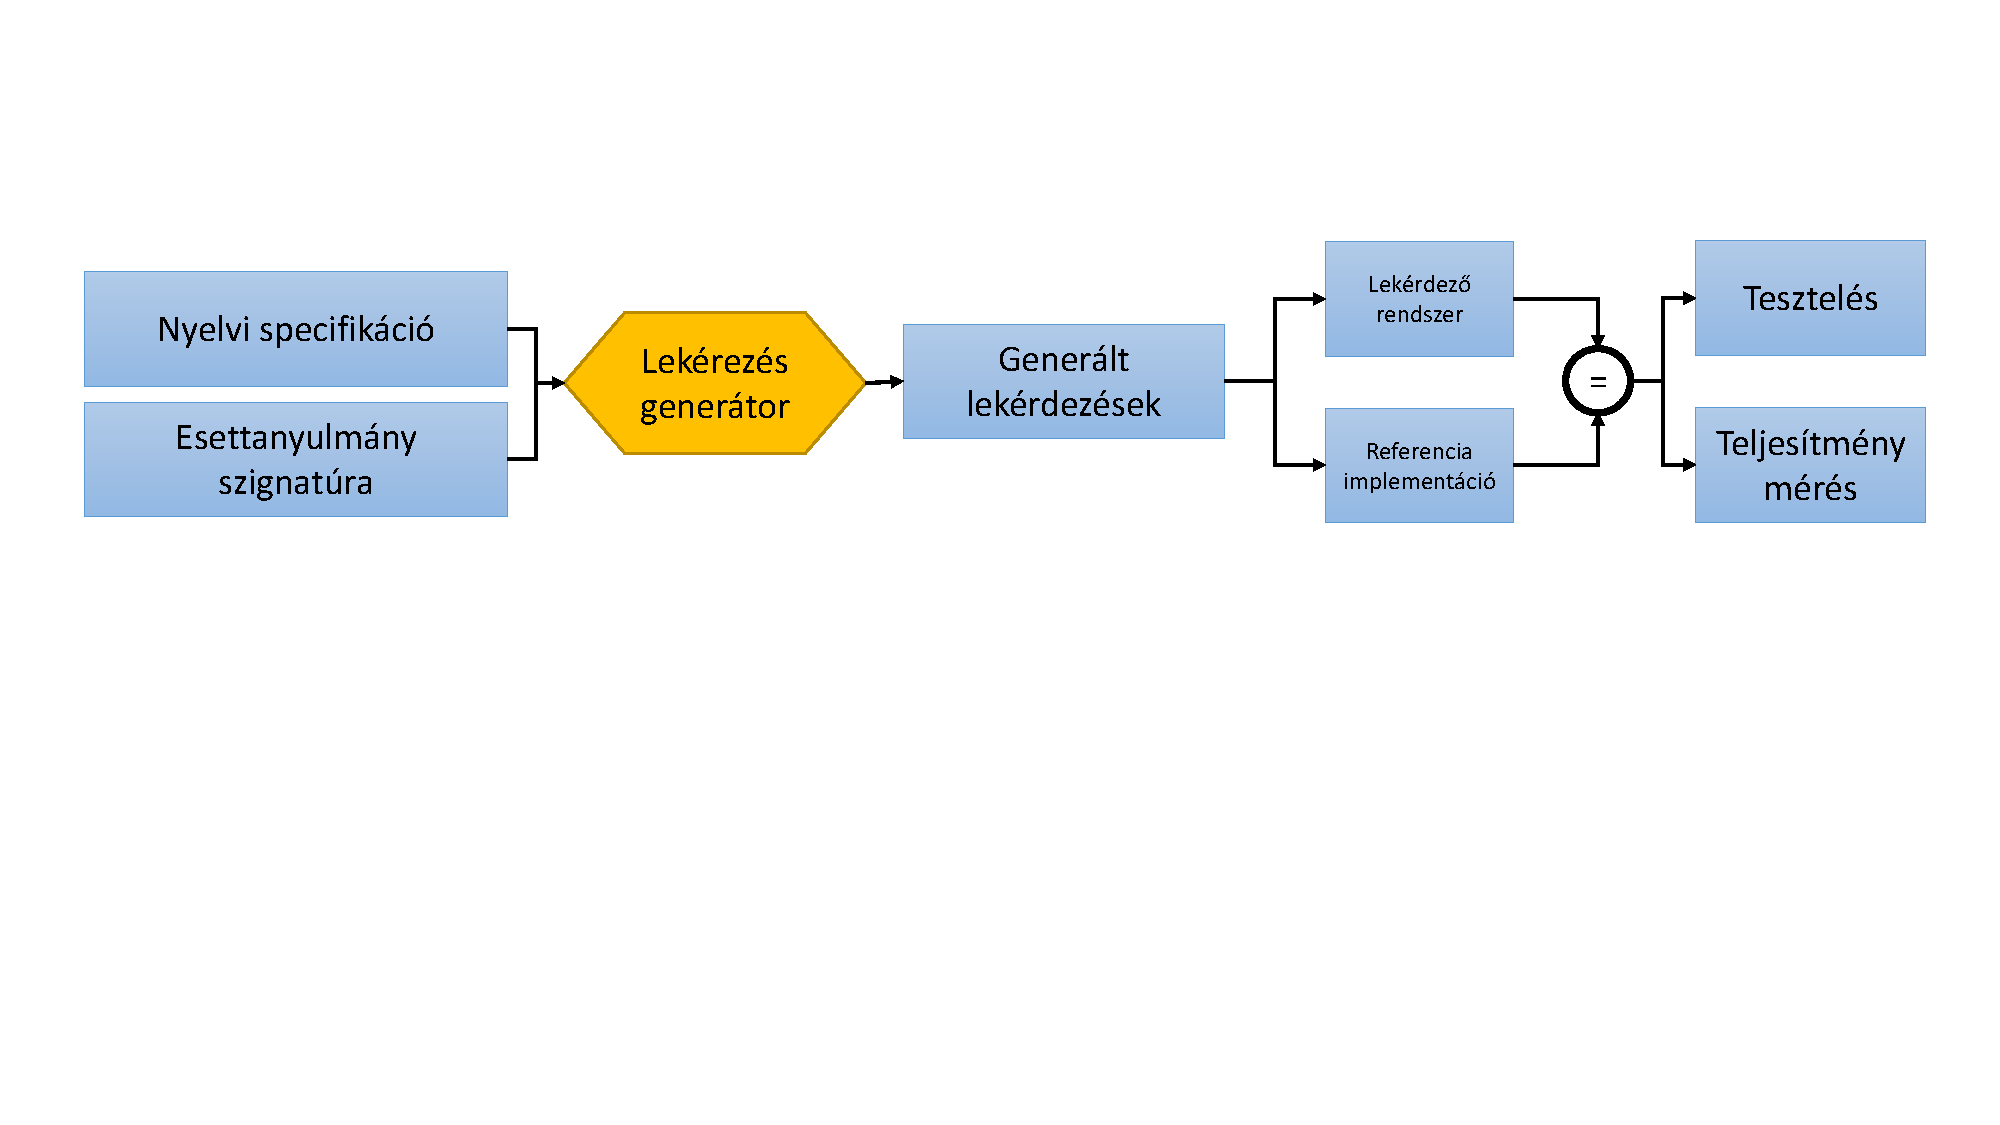
\includegraphics[width=1.0\textwidth]{figures/funkcionalisAttekintes}
	\caption{Az elképzelés funkcionális áttekintése}
	\label{fig:funkcionalisAttekintes}
\end{figure}
 
  

\section{Lekérdezés generálási folyamat felépítése}


A folyamat felépítését \aref{fig:blokkdiagramAttekintes} -es ábra segítségével ismertetem.  

\begin{figure}
	\centering
	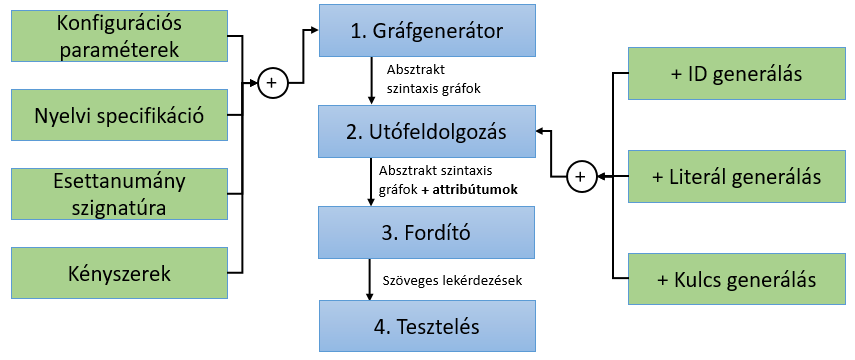
\includegraphics[width=1.0\textwidth]{figures/blokkdiagramAttekintes}
	\caption{A lekérdezés generálási folyamat áttekintése}
	\label{fig:blokkdiagramAttekintes}
\end{figure}
\begin{enumerate}
	\item \textbf{Gráfgenerátor}
	A gráf generálást a Viatra Solver keretrendszer  segítségével végzem. Ehhez sok különböző bemenetet kell megadnom. 
	\begin{enumerate}
		\item\textbf{Nyelvi specifikáció}: A Cypher nyelv specifikációját tartalmazó metamodell a nyelv egészére kiterjed. Így lekérdezéseken kívül sok egyéb műveletet is definiál, mint például létrehozás, törlés. Olyan kényelmi, extrafunkcionális elemeket is tartalmaz amelyek csak bonyolítják a lekérdezéseket, hogy felhasználóbarátabban adhassák vissza a tartalmat, például a visszatérési referencia átnevezése \cypherStyle{(x AS "username")}. Ahhoz, hogy egyszerű lekérdezéseket generáljak nem szükséges ezt a hatalmas metamodellt feldolgozni, viszont egyértelműen meg kell határozni egy olyan részmodelljét, amelyből hiánytalanul előáll az egyszerű lekérdezések nyelvi specifikációja, továbbá a lényegtelen elemek szűrésével a generált modellsereg diverzitását is növeljük, mert így lényeges modellelemek között kell hogy különbözzenek. 
		\item\textbf{Kényszerek}: Azonban vannak	olyan szabályok amelyeket a metamodell nem tud kifejezni, betartásuk nélkül viszont a generált példánygráfok nem értelmezhetőek Cypher nyelvű lekérdezésekként. Például annak meghatározása, hogy milyen változókra lehet, és milyenekre nem lehet hivatkozni a visszatérési értékben. Ezeket a szabályokat jólformáltsági kényszerekkel tartatom be. 
		\item\textbf{Konfigurációs paraméterek}: A generátor működéséhez elengedhetetlen a saját nyelvén íródott konfigurációs fájl. Itt határozható meg, hogy milyen megoldóval működjön a generálás, hogy hányat használjon az egyes elemekből a generálás során, hogy mekkora és milyen mennyiségű példányokat generáljon stb.  
		\item\textbf{Esettanumány szignatúra}: A generált példánygráfok változók nélkül jönnek létre. Ahhoz, hogy egy értelmes adatbázison végezhessük el őket, fontos hogy fel legyenek fegyverezve az adatbázisban használt címkékkel, típusokkal. Mivel én a Train Benchmark által használt adatbázison futtattam lekérdezéseimet, ezért az általa használt szignatúrával szereltem fel a rendszert. 
	\end{enumerate}
	\item \textbf{Utófeldolgozás}: Az általam generált gráfokban a változóknak nem adok nevet. Megtehetném, hogy a generálás során kitöltöm őket, de csak úgy, hogy a gráfgenerátor a generált szavakat különbségekként kezelje két példánygráf között. A nagyobb diverzitás elérésének érdekében a generátor nem foglalkozik a változók elnevezésével. Az utófeldolgozás során az Esettanulmány szignatúra szavaival töltöm fel az addig még csonka példánygráfokat. (a) \textbf{ID-kel}, (b) \textbf{Literálokkal}, (c) \textbf{Kulcsokkal} és (d) \textbf{Címkékkel}.   
	\item \textbf{Fordító}: Az utófeldolgozás során sorosíthatóvá vált példány gráfokat a Cypher nyelv XText nyelven íródott nyelvtanának segítségével szöveges lekérdezésekké alakítom. 
	\item \textbf{Tesztelés}: Az így elkészült lekérdezések már használhatóak teljesítménymérésre és tesztelésre.
\end{enumerate}



